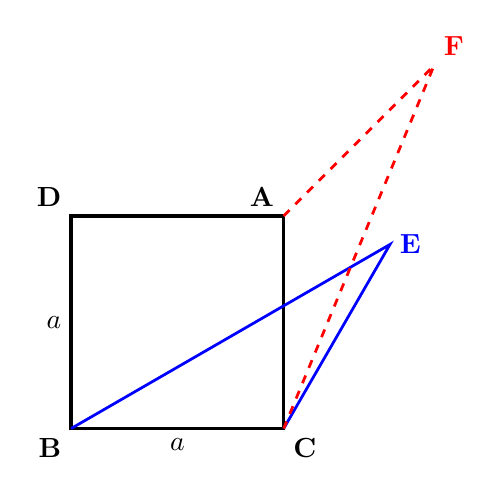
\begin{tikzpicture}[scale=0.9]
        % Square ABCD
        \draw[line width=1.2pt] (0,0) coordinate (B) -- (3,0) coordinate (C) -- (3,3) coordinate (A) -- (0,3) coordinate (D) -- cycle;
        
        % Diagonal AC
        \draw[thick, dashed] (A) -- (C);
        
        % Equilateral Triangle on side BC (BCE)
        \coordinate (E) at (4.5, 2.598);
        \draw[line width=1pt, blue] (B) -- (E) -- (C);
        
        % Equilateral Triangle on diagonal AC (ACF)
        % Angle of AC is -45 deg, side is 3*sqrt(2) = 4.242
        \coordinate (F) at (5.121, 5.121);
        \draw[line width=1pt, red, dashed] (A) -- (F) -- (C);
        
        % Labels
        \node[above left] at (D) {\textbf{D}};
        \node[above left] at (A) {\textbf{A}};
        \node[below left] at (B) {\textbf{B}};
        \node[below right] at (C) {\textbf{C}};
        \node[right, blue] at (E) {\textbf{E}};
        \node[above right, red] at (F) {\textbf{F}};
        
        % Side labels
        \node[below] at (1.5,0) {$a$};
        \node[left] at (0,1.5) {$a$};
    \end{tikzpicture}
